\section{Poisson solver}
\label{sec:poisson}
\renewcommand{\thesubsection}{\thesection.\arabic{subsection}}
In this section of the lab report, we will dicuss a prallel implementation of the Poisson solver. The Poisson solver is a numerical method used to solve the Poisson equation, which is a partial differential equation that is useful in many areas of physics. \\
\textbf{Note:} For local testing and development I'll run the code with \texttt{mpirun} instead of the \texttt{srun} command on the cluster. \\

\subsection{Building a parallel Poisson solver}
For the first part of the exercise we follow the steps lined out in the assignment sheet. I'll comment on the steps 1 through 10 and related questions bellow. The finished implementation can be found in the appendix for this section. \\
\begin{enumerate}
    \item \textbf{Step:} After adding MPI\_Init and MPI\_Finalize, we can run the program with multiple processes. We can see that the program runs with 4 processes in \autoref{fig:poisson_step1} via the quadrupeled output.
    \begin{figure}[H]
        \centering
        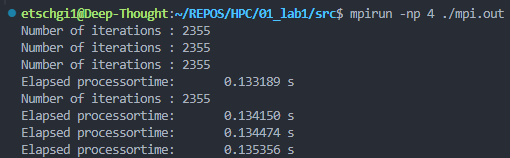
\includegraphics[width=0.5\textwidth]{../fig/lab1/step1.png}
        \caption{MPI\_Poisson after Step 1 - Running with 4 processes}
        \label{fig:poisson_step1}
    \end{figure}
    \item \textbf{Step:} To see which process is doing what, I included the rank of the process for the print statements as shown in \autoref{fig:poisson_step2}.
    \begin{figure}[H]
        \centering
        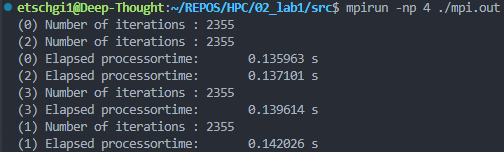
\includegraphics[width=0.5\textwidth]{../fig/lab1/step2.png}
        \caption{MPI\_Poisson after Step 2 - Running with 4 processes}
        \label{fig:poisson_step2}
    \end{figure}
    \item \textbf{Step:} Next we define \texttt{wtime} as a global double and replace the four utility timing functions with the ones given on Brightspace. A quick verification as shown in \autoref{fig:poisson_step3} shows that the program still runs as expected.
    \begin{figure}[H]
        \centering
        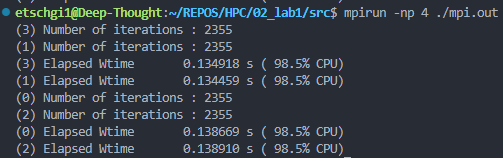
\includegraphics[width=0.5\textwidth]{../fig/lab1/step3.png}
        \caption{MPI\_Poisson after Step 3 - Running with 4 processes}
        \label{fig:poisson_step3}
    \end{figure}
    \item \textbf{Step:} Next we check if two processes indeed give the same output. Both need 2355 iterations to converge and the \texttt{diff} command returned no output, which means that the files content is identical. 
    \item \textbf{Step:} Now only the process with rank 0 will read data from files and subsequently broadcast it to the others. Testing this again with 2 processes, we see an empty diff of the output files and the same number of iterations needed to converge.
    \item \textbf{Step:} We create a cartesian grid of processes using \texttt{MPI\_Cart\_create} and use \texttt{MPI\_Cart\_shift} to find the neighbors of each process. We can see that the neighbors are correctly identified in \autoref{fig:poisson_step6}. 
    \begin{figure}[H]
        \centering
        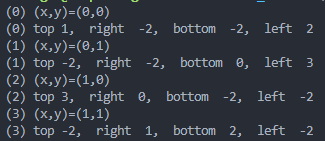
\includegraphics[width=0.5\textwidth]{../fig/lab1/step6.png}
        \caption{MPI\_Poisson after Step 6 - Running with 4 processes on a 2x2 grid}
        \label{fig:poisson_step6}
    \end{figure}
    When there is no neighbor in a certain direction, -2 (or \texttt{MPI\_PROC\_NULL}) is returned. 
    \item \textbf{Step:} We overhaul the setup to get a proper local grid for each process. Furthermore, we only save the relevant source fields in the local grid for each process. \\
    \Shining{With for instance 3 processes you should see that 1 or 2 processes do not do any 
    iteration. Do you understand why?}\\
    If we have a look at the input file we see that there are only 3 source fields in the grid. This means that the process that does not have a source field in its local grid will not do any iterations (or only 1). Therefore, if we have 3 processes and the distribution of source fields as given in the input file only 1 process will do iterations if processes are ordered in x-direction and 2 if ordered in y-direction. From this we can conclude that indeed all processes have different local grids and perform different calculations. 
    \begin{figure}[H]
        \centering
        \begin{minipage}{0.48\textwidth}
            \centering
            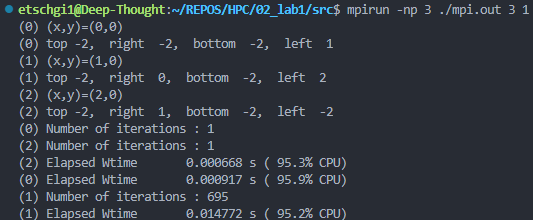
\includegraphics[width=\linewidth]{../fig/lab1/step7a.png}
        \end{minipage}%
        \hspace{0.02\textwidth}
        \begin{minipage}{0.48\textwidth}
            \centering
            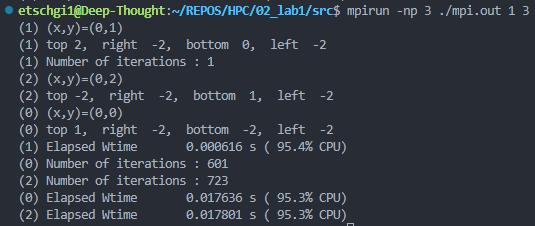
\includegraphics[width=\linewidth]{../fig/lab1/step7b.png}
        \end{minipage}
        \caption{MPI\_Poisson after Step 7 - Running with 3 processes on a 3x1 (left) vs. 1x3 (right) grid\\For the 3x1 grid, only rank 1 does iterations ($> 1$), for the 1x3 grid, ranks 0 and 2 do iterations ($> 1$).}
        \label{fig:poisson_step7}
    \end{figure}
    \item \textbf{Step:} After defining and commiting two special datatypes for vertical and horizontal communication, we setup the communication logic to exchange the boundary values between the processes. We call our \texttt{Exchange\_Borders} function after each iteration (for both red / black grid points). Now we face the problem in which some processes may stop instantly (no source in their local grid). They will not supply any data to their neighbors, which will cause the program to hang. We shall fix this in the next step.
    \item \textbf{Step:} Finally we need to implement the logic to check for convergence (in a global sense). We do this by using a \texttt{MPI\_Allreduce} call with the \texttt{MPI\_MAX} operation. This way we aggregate all deltas and choose the biggest one for the global delta which we use in the while-loop-condition to check for convergence. We can see that the program now runs as expected in \autoref{fig:poisson_step9}.
    \begin{figure}[H]
        \centering
        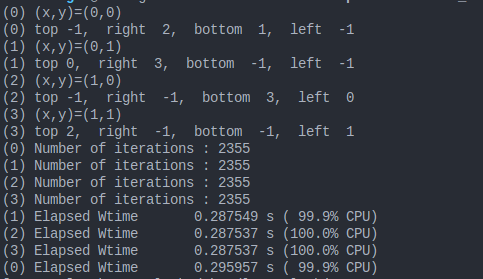
\includegraphics[width=0.5\textwidth]{../fig/lab1/step9.png}
        \caption{MPI\_Poisson after Step 9 - Running with 4 processes on a 2x2 grid}
        \label{fig:poisson_step9}
    \end{figure}
    Note that this run in \autoref{fig:poisson_step9} was done with another pc and another MPI implementation. Therefore, we see $-1$ for cells without a neighbor! However, other than that cosmetic difference it has no impact on the programm. 
    \item \textbf{Step:} Now we only have to fix two remaining things. First we have to make sure that each process uses the right global coordinates for the output file in the end. Therefore, we change the function a bit to include the specific x-/y-offset for each processor. The second thing is the potential problem, that different processors might start with different (red/black) parities. In order to accomplish a global parity we simply have to change the calculation in the if in \texttt{Do\_Step} from 
    \begin{lstlisting}[language=c, lastline=1]
        if ((x + y) % 2 == parity && source[x][y] != 1)
    \end{lstlisting}
    to
    \begin{lstlisting}[language=c, lastline=1]
        if ((x + offset[X_DIR] + y + offset[Y_DIR]) % 2 == parity && source[x][y] != 1)
    \end{lstlisting}
    this guarantees that during a given iteration all processors are using the same parity. 
\end{enumerate}
This just leaves one question open: Are the results acutally the same?\\
Checking the output files of the MPI-implementation with the sequential reference indeed shows identical numerical values for the calculated points. Furthermore, the needed iterationcount is also identical which isn't a big surprise, given that the two programms perform the exact same calculation steps. 
\subsection{Exercises, modifications, and performance aspects}
For this subsection we'll define the following shorthand notation: \\

\begin{table}[h!]
    \centering
    \begin{tabular}{|l|l|}
        \hline
        $n$:  &the number of iterations\\\hline
        $g$:  &gridsize\\\hline
        $t$:  &time needed in seconds\\\hline
        $pt$: & processor topology in form $pxy$, where:\\
        $p$:  &number of processors used\\
        $x$:  &number of processors in x-direction\\
        $y$:  &number of processors in y-direction\\\hline
       \end{tabular}
    \caption{Notation for this section}
\end{table}
$pt = 414$ means 4 processors in a $1\times 4$ topology. 

\subsubsection{Over-relaxation (SOR)}
We start of by rewriting the \texttt{Do\_Step} routine to facilitate SOR updates. Furthermore, we need $h^2$, the grid spacing (which is 1 in our case) and the relaxation parameter $\omega$ to calculate the updated values. A quick test shows a speedup of roughly a factor of 10. More systematic tests will be done in the next section.
\subsubsection{Optimal $\omega$ for 4 proc. on a 4x1 grid}
With the power of a little python scripting we can easily test different values for $\omega$ and plot the results as seen in \autoref{fig:best_omega_122}. 

\begin{figure}[H]
    \centering
    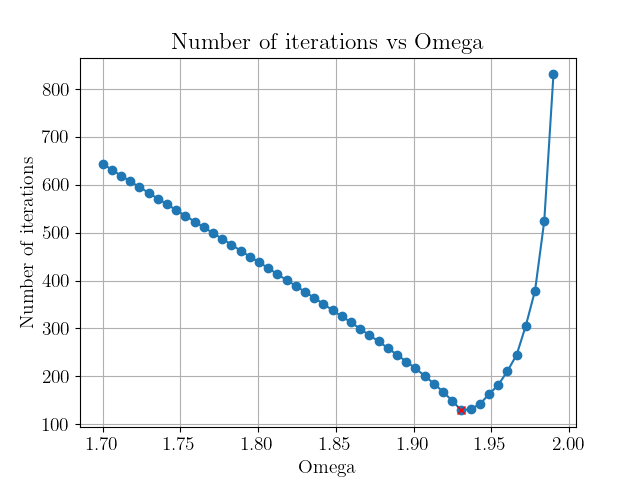
\includegraphics[width=0.7\textwidth]{../fig/lab1/best_omega_122.png}
    \caption{\Shining{Optimal $\omega$ for 4 processors on a 4x1 grid}}
    \label{fig:best_omega_122}
\end{figure}
We find that the optimal $\omega$ is at about $1.93$ for this setup with only 129 iterations. This constitutes a speedup of about 1825\% compared to the sequential implementation.

\subsubsection{Scaling behavior with larger grids}
This investigation is carried out twice: Once with a $4\times 1$ topology (as in the previous section) and once with a $2\times 2$ topology. We use grid sizes of $10\times 10$, $25\times 25$, $50\times 50$, $100\times 100$, $200\times 200$, $400\times 400$, $800\times 800$ and $1600\times 1600$ and set $\omega = 1.95$ for all runs. The results are shown in \autoref{fig:scaling_123}.

\begin{figure}[H]
    \centering
    \begin{minipage}{0.48\textwidth}
        \centering
        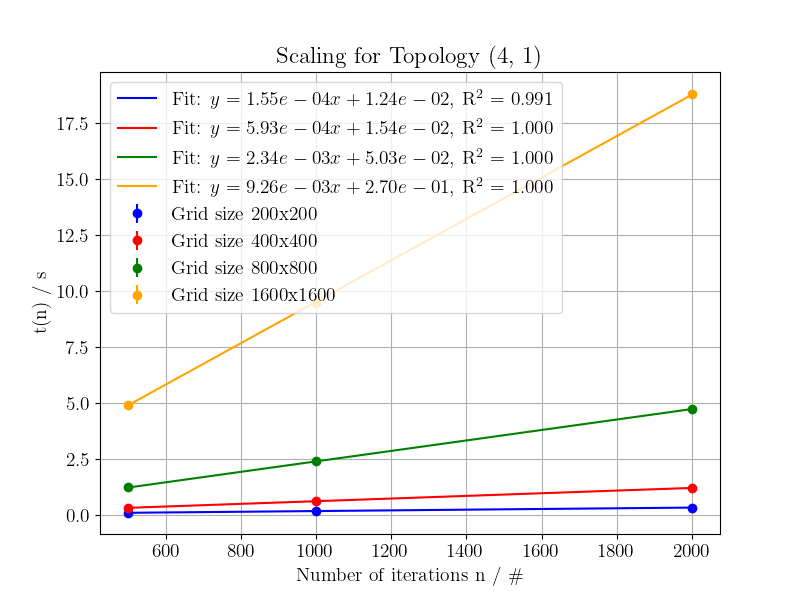
\includegraphics[width=\linewidth]{../fig/lab1/scaling_topology_4x1.png}
    \end{minipage}%
    \hspace{0.02\textwidth}
    \begin{minipage}{0.48\textwidth}
        \centering
        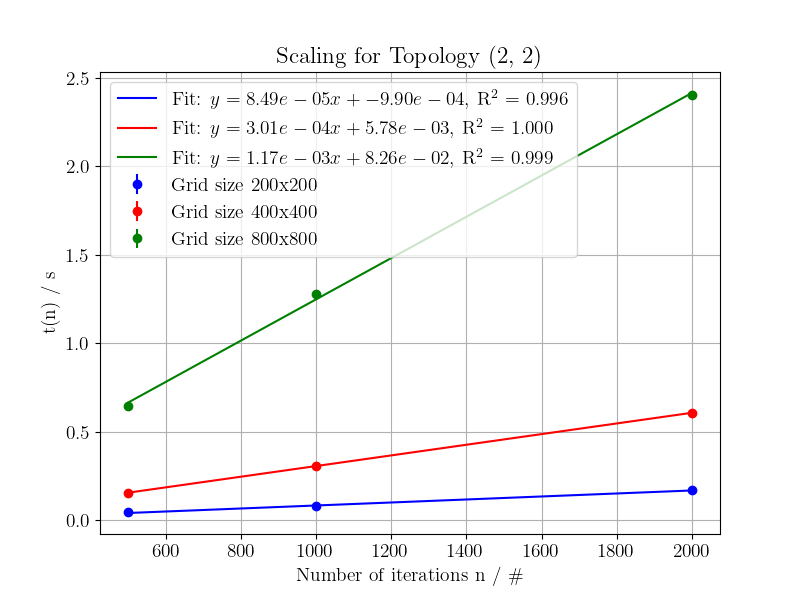
\includegraphics[width=\linewidth]{../fig/lab1/scaling_topology_2x2.png}
    \end{minipage}
    \caption{Scaling behavior of the Poisson solver with different grid sizes and processor topologies}
    \label{fig:scaling_123}
\end{figure}
As seen by the high $R^2$ values in the plots, the scaling behavior is very close to linear. 
We obtain the following scaling factors for the different grid sizes and topologies from the linear fits:
\begin{table}[H]
    \centering
    \begin{tabular}{|c|c|c|}
        \hline
        Topology & $\alpha$ & $\beta$ \\\hline
        $4\times 1$ & $1.35+10^{-1}$ & $7.11+10^{-6}$ \\\hline
        $2\times 2$ & $1.06+10^{-1}$ & $6.17+10^{-6}$ \\\hline
    \end{tabular}
    \caption{Scaling factors for different processor topologies for the Poisson solver\\Using: $t(n) = \alpha + \beta \cdot n$ as a model}
\end{table}
\Shining{What can you conclude from the scaling behavior?}\\
We see that the scaling behavior is very close to linear for both topologies. This means that the parallel implementation scales as expected with the number of grid points.\\
If we compare the scaling factors ($\beta$) for the two topologies we see that the $2\times 2$ topology scales slightly better than the $4\times 1$ topology. This is not surprising, as the $2\times 2$ topology has a more balanced communication workload balance. In the $2\times 2$ topology every processor has two neighbors, while in the $4\times 1$ topology the processors at the ends only have one neighbor. This is a general trend: A topology which divides the grid into square / square-like parts will scale better than a topology which divides the grid into long and thin parts.\\
In essence: We want to keep the communication between processors as balanced as possible to achieve the best scaling behavior.